\Chapter{Case data}
The population projection visualized in this project have been created by a geosimulation, which geographically distribute the predicted population. This geosimulation have been run every tenth year from 2010 to 2100. It has also been run for different scenarios for the feature.
\section{The data behind the simulation}
This projection is a geographical distribution of the global prospects created by The United Nations Department of Economic and Social Affairs. These prospects estimate the population numbers in each country living in rural and urban areas. The spatial distribution has been based on raster data from the Global Rural Urban Mapping Project (GRUMP). In this dataset the world has been divided into 1x1 km cell, each of which contains the number of estimated people. 
GRUMP also have a dataset for the extent of urban areas. This urban extent has been estimated based on the light emitted after dark, which as a result means that it overestimates the extent of urban areas. To compensate for this the dataset was combined with the Global Land Cover Map from the European Space Agency (GlobCover). This dataset more accurately defines the extent of urban areas. Only the areas which qualified as urban in GRUMP dataset and were classified as “artificial surfaces and associated urban areas” in the GlobCover data were treated as urban areas. 

\section{The simulation}
Using this dataset to define the extent of urban, suburban, and rural areas, the simulation was run as illustrated in figure \ref{CreatingData}

\begin{figure} [H]
	\centering
	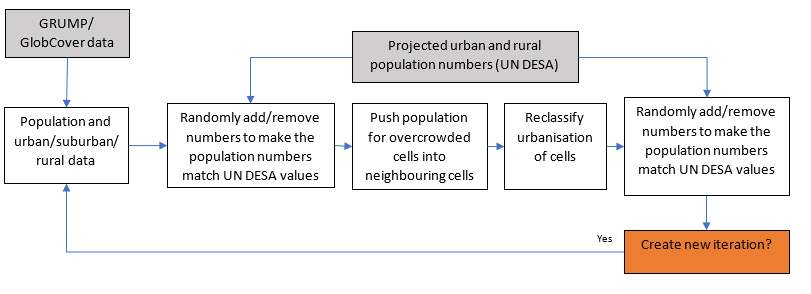
\includegraphics[width=.8\textwidth]{Pictures/CreatingData}
	\caption{A flowdiagram of simulation creating the population projections}
	\label{CreatingData}
\end{figure}

The population in rural and urban areas were adjusted to match the projected values from UN DESA. This was done by randomly adding or removing people from the area types. 

The cells would have a country-specific limit on how many people could live in them. Any cells with a population above this limit would push the excess population to neighboring cells. 

After this, the cells would be reclassified as more urbanized if their population had increased above a country-determined threshold. This way a rural cell might become a suburban one or a suburban become urban if its population increased. The data is then adjusted to match projected values again with the same approach as before. This is required because the reclassification would mean that the number for the different urbanization classes would no longer match the numbers from UN DESA.

These steps are then repeated for every iteration. 


\section{Shared Socioeconomic Pathways}


\fxnote{Create own figure}

The geosimulation have been run for five different future scenarios called the Shared Socioeconomic Pathways (SSPs). The different scenarios are based on different ways, climate change could affect society. As illustrated in figure x the five scenarios are based on two axes: socio-economic challenges for mitigation and for adaptation of climate change impacts. 
“Socio-economic” is referring to a large array of societal and socioecological system. Covering aspects of a political, social, demographic, cultural, lifestyle, institutional, economic, and technological nature and condition of ecosystems. 
The horizontal axis is environmental or societal conditions, which would make adapting to climate change more difficult. This include climate hazards (temperature and precipitation changes, sea level rise and extreme weather phenoms); what and whom these hazards will affect.
\citep{ConceptSSP}
The vertical axis is factors, which in absence of climate policy would increase that amount of emissions of greenhouse gasses and factors reducing the society’s capacity to lessen those emissions. Examples of factors reducing society’s capacity is inadequate technologies and insufficient resources to support mitigation policies. The increase in greenhouse gasses could for example be a result of population and economic growth.
\citep{SSP}

\begin{table}[htbp]
	\centering
	\begin{tabular}{l}
		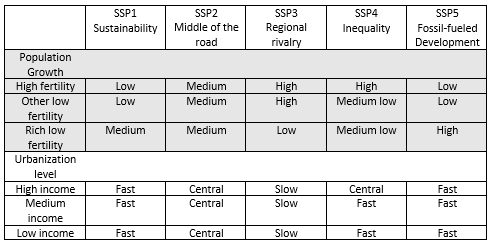
\includegraphics[width=0.8\textwidth]{Pictures/SSPTable}
	\end{tabular}
	\caption{Population growth and urbanization for each of the SSPs}
	\label{SSPTable}
\end{table}

How the population growth and the urbanization levels will be in the different scenarios can be seen in table \ref{SSPTable}. This table have been created by \citet{MaybeSEDAC}. The population growth values are based on current income and fertility condition. The urbanization predictions are based on the current income.

\fxerror{Need more context to the table - what does it mean? Do I need it? - use it to select what to show in results}

\section{Technical details about the case data}

\fxnote{Write this - leads to the next section}